\documentclass[
aip,
apl,
twocolumn,
secnumarabic,
graphicx,
reprint,
amsmath,
amssymb,
%draft,
]{revtex4-2}

%% SAND-BOXING
%\linenumbers\relax % Commence numbering lines
\usepackage{todonotes}
\usepackage[export]{adjustbox}

%% GRAPHICS
%\graphicspath{{../Master_Files/Figures/}}
%\DeclareGraphicsExtensions{.png,.pdf}
\pdfinclusioncopyfonts=1

%% TABLES
%\usepackage{booktabs}
\usepackage{dcolumn}% Align table columns on decimal point

%% LISTS
\usepackage[inline,shortlabels]{enumitem}

%% CHEMISTRY
\usepackage[version=4]{mhchem}  % for setting chemical formula with \ce{}
\usepackage{siunitx}					% for instance, \SI{0.1}{\nm} and \num{2}
\DeclareSIUnit \molar {\mole\per\cubic\deci\metre}
\DeclareSIUnit \Molar {\textsc{m}}
\DeclareSIUnit \G {G_0}
\DeclareSIUnit \angstrom {\textsc{\AA}}

\usepackage{chemmacros}				%this is for \iupac{} chemical names
\usepackage{chemfig}
\setchemfig{atom sep = 0.8 em}
\setchemfig{bond offset = 0 em}
\setchemfig{bond style={line width=1pt}}

% chemicals
\newcommand{\SAc}{\iupac{thio|acet|ate}}
\newcommand{\ope}{\iupac{oli|go-phen|ylene ethyn|ylene}}
\newcommand{\OPE}{\iupac{Oli|go-phen|ylene ethyn|ylene}}
\newcommand{\odt}{\iupac{oct|ane|di|thiol}}
\newcommand{\ODT}{\iupac{Oct|ane|di|thiol}}
\newcommand{\aDT}{\iupac{alk|ane|di|thiol}}
\newcommand{\ADT}{\iupac{Alk|ane|di|thiol}}
\newcommand{\bpy}{\iupac{4,4'-bi|pyri|dine}}
\newcommand{\pyr}{\iupac{pyri|dine}}
\newcommand{\thf}{\iupac{tetra|hydro|furan}}
\newcommand{\drawOPE}{\chemfig{HS-*6(-=-(-~-*6(-=-(-~-*6(-=-(-SH)=-=))=-=))=-=)}}
\newcommand{\drawBPY}{\chemfig{[:-30]N*6(-=-(-*6(-=-N=-=))=-=)}}
\newcommand{\drawODT}{\chemfig{HS-[:30]-[:-30]-[:30]-[:-30]-[:30]-[:-30]-[:30]-[:-30]-[:30]SH}}
\newcommand{\silane}{\iupac{sil|ane|di|thio|methyl}}
\newcommand{\Silane}{\iupac{Sil|ane|di|thio|methyl}}
\newcommand{\SH}{\iupac{thi|ol}}
\newcommand{\NHH}{\iupac{am|ine}}
\newcommand{\alkane}{\iupac{alk|ane}}
\newcommand{\Alkane}{\iupac{Alk|ane}}
\newcommand{\ferrocene}{\iupac{fe|rroc|ene}}
\newcommand{\metalorganic}{\iupac{me|tal|or|gan|ic}}

%% ACRONYMS
\usepackage[nolist,nohyperlinks]{acronym}
% Definitions are \input after \maketitle

\newcommand{\citetemp}[1]{\textcolor{red}{(#1)}}
\newcommand{\qtytemp}[1]{\textcolor{orange}{(#1)}}

%% definitions specific to this MS
\newcommand{\bpycoldnum}{\num{\approx 3900} }
\newcommand{\bpycoldnummol}{\num{\approx 2000} }
\newcommand{\bpycoldnumtun}{\num{\approx 1900 } }
\newcommand{\bpyrtnum}{\num{\approx 9800 } }
\newcommand{\sinum}{\num{\approx 20000 } }
\newcommand{\sinummol}{\num{\approx 14000 } }
\newcommand{\sinumtun}{\num{\approx 6000 } }

%%%%%%%%%%%%%%%%
% End preamble, begin document
%%%%%%%%%%%%%%%%


\begin{document}

\title{Single molecular break junction break point detection: There and back again}

\newcommand{\UCPH}{Department of Chemistry, University of Copenhagen, Universitetsparken 5, 2100 Copenhagen}
\author{Joseph M. Hamill}
%\email{j.m.hamill@bham.ac.uk}
\email{jmh@chem.ku.dk}
\affiliation{\UCPH}

\author{William Bro-J\o{}rgensen}
\affiliation{\UCPH}

\author{Gemma C. Solomon}
\email{gsolomon@chem.ku.dk}
\affiliation{\UCPH}

\date{\today}

\begin{abstract}
We present \ac{cpd} as an alternative to the growing interest in \acl{ml} methods to study \acl{smbj} data sets. We apply \ac{cpd} to three separate data sets, two on \acl{bpy} and one on silane, two at \acl{rt} and one at \qty{4}{\K}, two in one lab, one in another, to show the wide applicability of even the most simplistic of \ac{cpd} algorithms: the Chow test. We demonstrate that using \ac{cpd} instead of the conventional \acl{1DGH} to determine the mean molecular conductance yields a standard deviation in the estimate of typically half that of the conventional approach, meaning the estimate is known with better accuracy. This better accuracy propagates into more accurate theoretical simulations, which in turn are predicting Fermi alignments and thermal properties.
\end{abstract}

\pacs{}

\maketitle

%% Acronyms and definitions
%%Use this call in preample:
%\usepackage[nolist,nohyperlinks]{acronym}
%%\inlude these definitions after \maketitle (at least for REVTEX)
%%
\begin{acronym}[ACRONYM]
\acro{ct}[CT]{Catchy Title}
\acro{cpd}[CPD]{change point detection}
\acro{bp}[BP]{break point}
\acro{sm}[SM]{single-molecule}
\acro{smbj}[SMBJ]{single molecular break junction}
\acro{stm}[STM]{scanning tunneling microscope}
\acro{mcbj}[MCBJ]{mechanically controlled break junction}
\acro{bj}[BJ]{break junction}
\acro{iv}[IV]{current versus bias}
\acro{rt}[RT]{room temperature}
\acro{sam}[SAM]{self-assembled monolayer}
\acro{JMH}[JMH]{Dr. Joseph M. Hamill}
\acro{GCS}[GCS]{Prof. Gemma C. Solomon}
\acro{JOOJ}[JOOJ]{Prof. Jan O. O. Jeppesen}
\acro{ucph}[UCPH]{University of Copenhagen}
\acro{SG}[SG]{Solomon Group}
\acro{AH}[AH]{Prof. Andr\'{a}s Halbritter}
\acro{BME}[BME]{Budapest University of Technology and Economics}
\acro{NRL}[NRL]{Nano}
\acro{MHG}[MHG]{Marc Hamilton Garner}
\acro{rnn}[RNN]{recurrent neural network}
\acro{pca}[PCA]{principal component analysis}
\acro{uhv}[UHV]{ultra-high vacuum}
\acro{gap}[$\mathcal{G}$]{gap}
\acro{obj}[$\mathcal{O}$]{objective}
\acro{wp}[$\mathcal{W \mkern -7mu P}$]{work package}
\acro{EMRS}[E-MRS]{European Materials Research Society}
\acro{sota}[SOTA]{state-of-the-art}
\acro{odt}[ODT]{\odt}
\acro{ODT}[ODT]{\ODT}
\acro{bpy}[BPY]{\bpy}
\acro{thf}[THF]{\thf}
\acro{OPE3}[OPE3]{OPE3}
\acro{ope}[OPE]{\ope}
\acro{OPE}[OPE]{\OPE}
\acro{gmm}[GMM]{Gaussian mixture model}
\acro{3D}[3D]{three dimensional}\acused{3D}
\acro{adf}[ADF]{augemented Dickey-Fuller}
\acro{kpss}[KPSS]{Kwiatkowski–Phillips–Schmidt–Shin}
\acro{dfgls}[DFGLS]{augmented Dickey-Fuller with generalized least squares}
\acro{df}[DF]{Dickey-Fuller}
\acro{pp}[PP]{Phillips–Perron}
\acro{rss}[RSS]{residual sum of squares}
\acro{plh}[PLH]{plateau length histogram}
\acro{rms}[RMS]{root mean square}
\acro{itn}[ITN]{initial training network}
\acro{esr}[ESR]{early-stage researcher}
\acro{sdu}[SDU]{University of Southern Denmark}
\acro{ubern}[UniBern]{University of Bern}
\acro{ubham}[U. Birmingham]{University of Birmingham}
\acro{ml}[ML]{machine learning}
\acro{1DGH}[1DGH]{1D conductance histogram}
\acro{2DH}[2DH]{2D intensity plot}
\acro{daq}[DAQ]{data acquisition}
\acro{uroch}[U. Rochester]{University of Rochester}
\acro{JR}[JR]{Prof. Jascha Repp}
\acro{IF}[IF]{Prof. Ignacio Franco}
\acro{msca}[MSCA]{Marie Sk{\l}odowska-Curie Actions}
\acro{if}[IF]{Independent Fellowship}
\acro{qi}[QI]{quantum interference}
\acro{uregens}[U. Regensberg]{University of Regensberg}
\acro{JB}[JB]{Dr. James Bevington}
\acro{LAW}[LAW]{Dr. Luke A. Wilkinson}
\acro{ucl}[UCL]{University College, London}
\acro{uyork}[U. York]{University of York}
\acro{udurham}[U. Durham]{University of Durham}
\acro{LOD}[LOD]{Dr. Luke O'Driscoll}
\acro{SP}[SP]{Prof. Stergios Piligkos}
\acro{MP}[MP]{Prof. Michael Pittelko}
\acro{MBN}[MBN]{Prof. Mogens Br{\o}ndsted Nielsen}
\acro{dft}[DFT]{density functional theory}
\acro{cots}[COTS]{commercial off-the-shelf}
\acro{risk}[$\mathcal{R}$]{risk}
\acro{ms}[$\mathcal{M}$]{milestone}
\end{acronym}

%% Other abbreviations
% latin
\newcommand{\etal}{\textit{et al}}
\newcommand{\eg}{e.g.}
\newcommand{\ie}{i.e.} % Apparently, acronyms need to be defined after \maketitle...

\section{Introduction \label{sec:intro}}
There is a lot of recent interest in advanced data analysis methods applied to single molecular electronics measurements using \ac{ml}.\cite{Hamill2018, Cabosart2019, Vladyka2020, Lauritzen2018, Huang2020} Applications of machine learning methods clustering approaches have suggested there is interesting behavior within subsets of whole datasets which may be instructional to understanding the dynamics of \acp{smbj} -- dynamics such as molecule-electrode geometry and interactions and overall junction trajectories. Three stated goals are: 
\begin{enumerate*}[(i)]
\item reverse a historic trend, either real or perceived, of subjective influence on the data analysis (such as hand-selection of traces),\cite{Hamill2018}
\item provide scope for analyzing ever-increasing amounts of data, made possible in part by improved measurement quality,\cite{Albrecht2017, Lauritzen2018} and
\item address difficulties comparing experimental transport observables with theoretical transport models.\cite{Li2019}
\end{enumerate*}

The first goal has provided ample challenges. In attempts to appear transparent and objective, suggested \ac{ml} methods are becoming quite cumbersome.\cite{Cabosart2019, Vladyka2020, Huang2020, Fu2020, Bamberger2020} Although \ac{ml} is tantalizing, it comes with pitfalls and potentially introduces its own form of subjectivity.\cite{Bro2021} To train useful machines sensitive to molecular features, a great deal of windowing, filtering, and other data manipulations are proving necessary. Most methods also require some parameter tuning. Even simpler machines may be confounded by non-molecular features.\cite{Hamill2018}

One typical method for studying \ac{smbj} data is to create \acp{1DGH}. Fig.~\ref{fig:dummy} illustrates why this approach is flawed. Fig.~\ref{fig:dummy}(a) depicts an idealized \ac{smbj} trajectory and Fig.~\ref{fig:dummy}(b) depicts the measured conductance trace. Such a trace starts with the rupture of the Au-Au point contact [i]. The elongated Au electrodes snap-back yielding a drop in conductance much faster than the preamp can track [ii]. Once the preamp catches up, the conductance follows a tunneling decay trend unless a molecule incorporates into the junction. In the case a molecule is incorporated, the conductance plateaus [iii]. Ideally, the molecular junction reaches a fully-extended geometry before it ruptures [iv]. After the molecular junction ruptures, the conductance trace returns to a tunneling decay trend [v] until the noise floor of the instrument is reached [vi]. 
\begin{figure}[]%
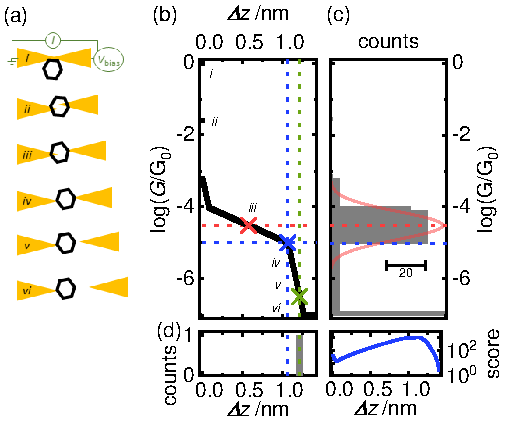
\includegraphics[width=\columnwidth,keepaspectratio,]{Fig_Dummy}
\caption{Idealized dummy trace and analysis. (b) An ideal trace following Au-Au rupture with [i] Au-Au contact, [ii] snap-back, [iii] molecular plateau, [iv] full extension, and [v] tunneling, and [vi] noise floor. Red X marks customary $\overline{G}_{mol}$; blue X marks molecular plateau \acs{bp}; green X marks point in trace where customary plateau length is determined. (c) 1D conductance histogram, gray, with Gaussian fit to determine $\overline{G}_{mol}$ in (b). (d) This trace produces a count in a \acs{plh} at the green mark.}%
\label{fig:dummy}%
\end{figure}

Historically, \ac{smbj} data was binned into a single summarizing \ac{1DGH},Fig.~\ref{fig:dummy}(c), which contains a peak if the trace contains a molecular plateau. In its time, this was an exciting outcome which allowed small molecular signals to appear out of data with low signal to noise ratios,\cite{Mayor2004} at the cost of losing time-dependent information. Customarily, the peak is fit to a Gaussian and the mean becomes the single summarizing parameter of the study. Too often, effectively something closer to the mode is used. Another common analysis step is to determine the displacement of the trace, Fig.~\ref{fig:dummy}(d), when it reaches a constant conductance, chosen at some value after the molecular plateau.

Here we emphasize that a fit to the \ac{1DGH} incorporates information about the entire molecular plateau, not just the fully-extended junction. In a highly downward sloping plateau, which is common for saturated molecular backbones\citetemp{cite discussion of plateau slope}, the mean will be considerably higher in conductance than the conductance of the fully extended junction, as depicted in Fig.~\ref{fig:dummy}(b) and (c). This results in an over-estimation of $\overline{G}_{\text{mol}}$. Furthermore, estimating the molecular plateau length by a measuring the distance to a point \textit{after} the molecular plateau ruptures will necessarily over-estimate it. Therefore, the determination of $\overline{z}_{\text{mol}}$ by fitting the \ac{plh}, Fig.~\ref{fig:dummy}(d), to a Gaussian will be an over-estimation. 

Critically, Fig.~\ref{fig:dummy} strongly suggests the third stated goal of recent \ac{ml} based advanced data analysis methods, to address difficulties comparing experiments with theory, will struggle to address these discrepancies, if they rely on the \ac{1DGH}. Due to limitations of computational time and resources, as well as of human time and resources, theory is typically calculated after optimizing a single, ideal geometry of the molecule situated perpendicularly between two electrodes.\citetemp{cite maybe a review} Work has been performed to understand and minimize the impact of the geometry of the electrodes.\citetemp{cite this, or remove it} The calculated transmission versus charge carrier energy describes, then, the transmission of electrons/holes through the one idealized geometry, or a handful of geometries, only. Next, the theorist may use a number of approximations to determine where the Fermi level of the electrode-molecule-electrode junction lies. One common tool is to return to the experimental data, specifically $\overline{G}_{\text{mol}}$ derived from the peak fit of the \ac{1DGH}, and align the experimental Fermi level with the appropriate energy to match $\overline{G}_{\text{mol}}$ of the experimental results. The result is that the theoretical interpretation of the energetics is also dependent on the experimentally determined $\overline{G}_{\text{mol}}$.

We propose directly determining the \ac{bp} of the molecular plateau to achieve better summaries of the experiment, and in turn, better comparison with theory. As an added benefit, in some cases, this approach may be both more accurate, and require far fewer traces.

\Ac{cpd} is a common task in econometrics, and there exist numerous methods for searching for structural breaks in data, accompanied by nuanced debate about which method is best.\cite{Truong2020} In there basic form, nearly all methods contain three elements:
\begin{enumerate*}[(i)]
	\item cost function,
	\item search method, and
	\item constraint.
\end{enumerate*}
For the purpose of this study, we are concerned with searching for a single structural break, or \ac{bp} in a \ac{smbj} trace, so the third item, constraint, is simply unity in our case. The choice of a search method must balance computation time with accuracy. For the purposes of this study, we will use the most basic of search methods: check each point in the (windowed) trace one at a time. This is a computationally expensive approach, and an alternative choice may improve this. Admittedly, we are starting with a worst case search method; if it works well, we can improve our search method. In this article we wish to focus on one particular choice of cost function: the Chow test. We have used the Chow test as a way to determining the \ac{bp} because it, too, is very simple.\cite{Chow1960} The Chow test tests whether a single linear regression of a time series is as good as the linear regressions of two segments created when the timeseries is divided at point $p$. In other words, we assume the timeseries, with $N$ elements, can be divided at index $p$ into two linear regressions,
\begin{equation}
	Y[1 \dots p] = a_1 \times X[1 \dots p] + b_1 + \varepsilon_1,
\end{equation}
and
\begin{equation}
	Y[p+1 \dots N] = a_2 \times X[p+1 \dots N] + b_2 + \varepsilon_2,
\end{equation}
which better describes the data than a single linear regression,
\begin{equation}
	Y[1 \dots N] = a_{\text{all}} \times X[1 \dots N] + b_{\text{all}} + \varepsilon_{\text{all}}.
\end{equation}
More specifically, the sum of the squared errors,\acused{rss}
\begin{equation}
	RSS_{1,2} = (\varepsilon_{1,2})^2,
\end{equation}
in these regressions are compared to \ac{rss} in the pooled regression, $\varepsilon_{\text{all}}$. For each $p$, the Chow score,
\begin{equation}
	f(p) = \frac{\sfrac{[RSS_{\text{all}} - (rss_1 + rss_2)]}{k}}{\sfrac{(RSS_1 + RSS_2)}{(N - 2k)}}
\end{equation}
is calculated, where $k$ is the number of parameters to fit ($k=2$ in our case: $a$ and $b$). The index where the Chow score is greatest,
\begin{equation}
	p_{\text{BP}} = \text{argmax}(f),
\end{equation}
is the index where \ac{rss} of the two linear regressions is smallest, and therefore the best estimate for the \ac{bp}. 

We begin by showing the Chow test applied to the idealized trace in Fig.~\ref{fig:dummy} to gain an intuition for how it behaves, starting with the whole trace in Fig.~\ref{fig:dummy_chow}(a). Interestingly, the Chow test identified a part of the trace following the \ac{bp}. Next the trace was thresholded to focus the test below \qty{}{10^{-4}~\G} (b), above \qty{}{10^{-6}~\G} (c), and both (d). Removing the snap-back region [Fig.~\ref{fig:dummy_chow}(b)] had little effect on the result of the Chow test, but removing the noise data at the end of the trace [Fig.~\ref{fig:dummy_chow}(c)] had a large adverse effect. Impressive results were achieved when the window was applied to both ends of the data [Fig.~\ref{fig:dummy_chow}(d)]. These tests suggested for most traces within a reasonable window, the Chow test will work well. 
\begin{figure}[]%
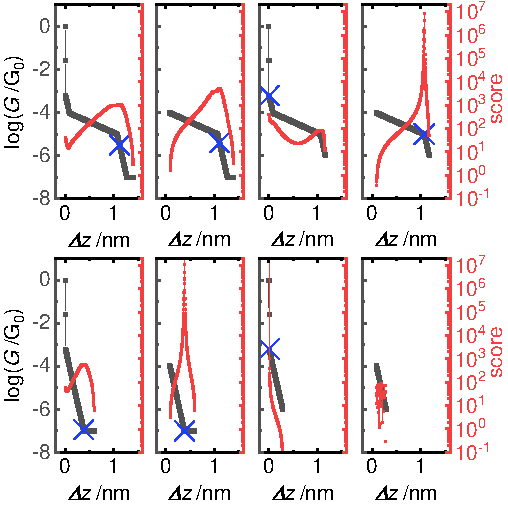
\includegraphics[width=\columnwidth,keepaspectratio,]{Fig_Dummy_Chow}
\caption{Chow score at each data point applied to dummy \ac{smbj} molecular [(a)-(d)] and tunneling [(e)-(h)] traces. (a) and (e) full traces; (b) and (f) traces windowed from above; (c) and (g) traces windowed from below; and (d) and (h) traces windowed from both sides.}%
\label{fig:dummy_chow}%
\end{figure}

On the bottom row [Figs.~\ref{fig:dummy_chow}(e)-(h)] the same windows were applied to an idealized blank trace. When no window was applied  [Fig.~\ref{fig:dummy_chow}(e)], the Chow test identified the inflection in the data when the trace reached the noise level. Likewise when the snap-back region was removed [Fig.~\ref{fig:dummy_chow}(f)]. When the noise level was removed [Fig.~\ref{fig:dummy_chow}(g)] the Chow test identified the inflection when the trace left the snap-back region. Finally, when both windows were applied [Fig.~\ref{fig:dummy_chow}(h)] the Chow test had no confidence in a \ac{bp}. 

%---------------------------------------------------------%
\section{Results and Discussion \label{sec:results}}
%---------------------------------------------------------%
%---------------------------------------------------------%
\subsection{Cryogenic and \acl{rt} data}
%---------------------------------------------------------%

The first cases we studied were \ac{bpy} measured at \qty{4}{\K} and \ac{rt}. It was expected that \qty{4}{\K} data would have sharp \acp{bp} and achieve good results applying the Chow test. Comparing \qty{4}{\K} with \ac{rt} data allowed us to make a comparison between "easy" data and "hard" data.

Fig.~\ref{fig:trace}(a) plotted a single example trace from a data set of \bpycoldnum traces of \ac{bpy} as analyte, of which \bpycoldnummol traces contained clear molecular features, based on a simple threshold filter of plateau slopes. The data was previously reported in Ref.~\onlinecite{Magyarkuti2020}. Based on the conclusions from the discussion around Fig.~\ref{fig:dummy_chow}, the trace was masked [grayed out regions in Fig.~\ref{fig:dummy_chow}(a)] to focus on conductances between \qty{}{10^{-2.4}~\G} and \qty{}{10^{-5.7}~\G}. Fig.~\ref{fig:trace}(b) plotted the Chow score tested at each data point in the range. The maximum Chow score, orange $\times$ in Fig.~\ref{fig:trace}(c), was slightly below the expected \ac{bp}. Fig.~\ref{fig:trace}(c) plotted the \ac{rss} for the entire trace segment (linear regression in light green and \ac{rss} in dark green), and the segment before/after the Chow score maximum (linear regression in light red/blue, and \ac{rss} in dark red/blue). 
\begin{figure}[]%
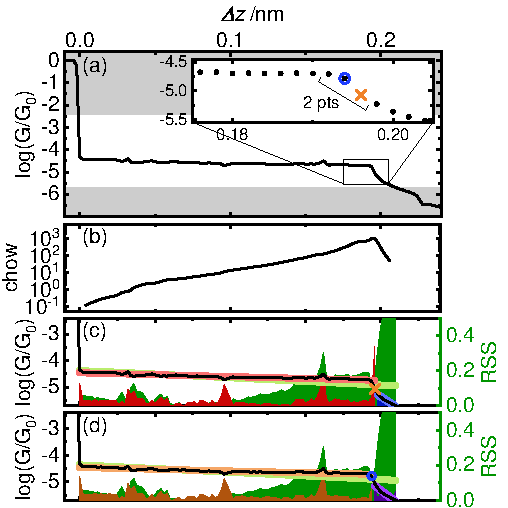
\includegraphics[width=\columnwidth,keepaspectratio,]{Fig_BPY_4K_trace}
\caption{Chow test applied to an example trace of \ac{bpy} measured at \qty{4}{\K}. (a) example conductance vs displacement trace; inset zoom in to end of molecular plateau with \ac{bp} determined by Chow test (orange $\times$) and Chow+ (blue circle); Chow+ searches \num{2} data points before the \ac{bp} chosen by the Chow test for the largest jump in conductance to determine an improved \ac{bp}. (b) Chow score vs data point for windowed region of trace. (c) linear regressions (pooled data in green, segment before \ac{bp} in red, and segment after \ac{bp} in blue) and \ac{rss} at \ac{bp} determined by Chow test. (d) linear regressions (pooled data in green, segment before \ac{bp} in orange, and segment after \ac{bp} in purple) and \ac{rss} at \ac{bp} determined by Chow+.}%
\label{fig:trace}%
\end{figure}

The lesson from Fig.~\ref{fig:dummy_chow} was that the exact choice of \ac{bp} determined by the Chow test may be skewed to lower conductances, likely a result of the particular search window. Because it was inefficient to choose a unique window for each trace, but instead one window for the entire data set, this lower skewing was predicted to alter the results of the Chow test method for determining the \ac{bp} for an entire data set. Another way to put this, the Chow test was a good and fast approach for searching globally for a region where the \ac{bp} was located. But to fine tune our result, we implemented a second step to the search. In this second step, we searched \num{2} data points before the \ac{bp} determined by the Chow test for the largest jump in the data, and chose the left data point in that jump. The inset in Fig.~\ref{fig:trace}(a) depicts such a search. The orange $\times$ marks the choice based solely on the Chow test; the blue $\bigcirc$ marks the choice after searching for the largest jump in the data. Fig.~\ref{fig:trace}(d) plotted the linear regressions and \ac{rss} for the new segments created by the new choice of \ac{bp}. The difference, in this case, was one data point, and there was little difference in the \ac{rss} between Figs.~\ref{fig:trace}(c) and (d). Fig.~\ref{fig:trace}(b), too, showed there was little difference between the Chow scores of the two points. Furthermore, the change in displacement between the two methods, one data point, was \qty{2.0}{\pm}. Yet, the change in conductance was not negligible: a change of \qty{0.6}{\nano\siemens}.

The \acp{bp} for all the molecular traces in the data set were then calculated, plotting both the simple Chow test (Chow, orange points) results and the Chow test plus correction (Chow+, blue points) results in Fig.~\ref{fig:BPY_cold}(a). A \ac{2DH} of only molecular traces was plotted in gray in Fig.~\ref{fig:BPY_cold}(a). The trace used in Fig.~\ref{fig:trace} was also plotted, with an red $\times$ at the Chow result, and a green $\bigcirc$ at the Chow+ result. The Chow results, without correction, yielded, on average, results much lower than where the molecular plateau appeared to end, but instead were located halfway down the break between the molecular plateau and the beginning of the noise level. On the other hand the Chow+ results, on average, appeared to be located just following the end of the molecular plateau. When the conductance of the \acp{bp} was plotted along with the 1D conductance histogram of the data set in Fig.~\ref{fig:BPY_cold}(d), the difference between $\overline{G}_{\text{mol}}$ from the Chow+ \ac{bp} and $\overline{G}_{\text{mol}}$ from the 1D conductance histogram was over a half order magnitude, a change of \qty{13.1}{\nano\siemens}\qtytemp{need to check this}. $\overline{z}_{\text{mol}}$ changed little between the conventional \ac{plh} and a histogram created from the displacements of the \acp{bp}, plotted in Fig.~\ref{fig:BPY_cold}(c). $\overline{G}_{\text{mol}}$ and $\overline{z}_{\text{mol}}$, as determined by Gaussian fits, for the \ac{1DGH}, Chow, and Chow+ were plotted in Fig.~\ref{fig:BPY_cold}(d), with the standard deviations used for error bars. It is noteworthy that the Chow+ approach reduced the standard deviation by half, compared to the conventional 1D histogram approach, meaning the accuracy with which $\overline{G}_{\text{mol}}$ is known was improved using Chow+ over the conventional method.
\begin{figure}[]%
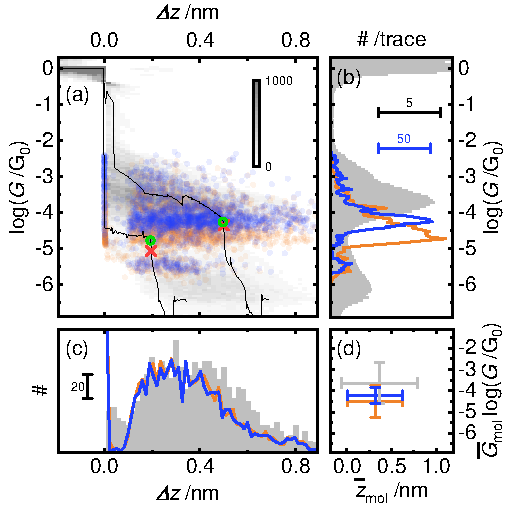
\includegraphics[width=\columnwidth,keepaspectratio,]{Fig_BPY_4K}
\caption{Chow test applied to \bpycoldnummol traces of \ac{bpy} at \qty{4}{\K}. (a) \ac{2DH} of all molecular traces in gray; scatter plots of Chow/Chow+ test choices of \ac{bp} (orange/blue); example trace with Chow/Chow+ \ac{bp} plotted in red/green. (b) Conductance histograms of all traces (gray), and conductance values of Chow/Chow+ test results (orange/blue). (c) Plateau length histogram (gray), and histograms of displacement values of Chow/Chow+ test results (orange/blue). (d) Mean of Gaussian fit to \ac{1DGH} of all data between \qty{}{10^{-1.0}~\G} and \qty{}{10^{-4.9}~\G} (gray) and \ac{plh}, and to conductances and displacements of Chow/Chow+ test results (orange/blue). Error bars are standard deviations.}%
\label{fig:BPY_cold}%
\end{figure}

Most \ac{smbj} experiments contain at least some tunneling traces which result when a molecule was not captured in the \acsu{bj}. The complete data set above contained \bpycoldnumtun traces which contained little or no molecular signal, as determined by the slope of the molecular region. To confirm the distribution of \acp{bp} in Fig.~\ref{fig:BPY_cold} was unique to the molecule, the tunneling traces were analyzed in an identical manner. A \ac{2DH} of the tunneling traces, overlayed with a scatter plot of \acp{bp}, determined with the Chow+ test, were plotted in Fig.~\ref{fig:tunnel_cold}(a). There was an intense region around \qty{}{10^{-5.5}~\G}, as confirmed by a histogram of conductance values, Fig.~\ref{fig:tunnel_cold}(b), which were likely marking the inflection of the trace from tunneling to noise, identical to the result on the dummy trace in Figs.~\ref{fig:dummy_chow}(e) and (f). This intense region was below the results for the molecular data in Figs.~\ref{fig:BPY_cold}(a) and (b). Indeed, there appeared to be some \acp{bp} with tunneling nature in the molecular data. A histogram of displacements, Fig.~\ref{fig:tunnel_cold}(c), helped to illustrate the distribution of displacements in the \acp{bp}.
\begin{figure}[]%
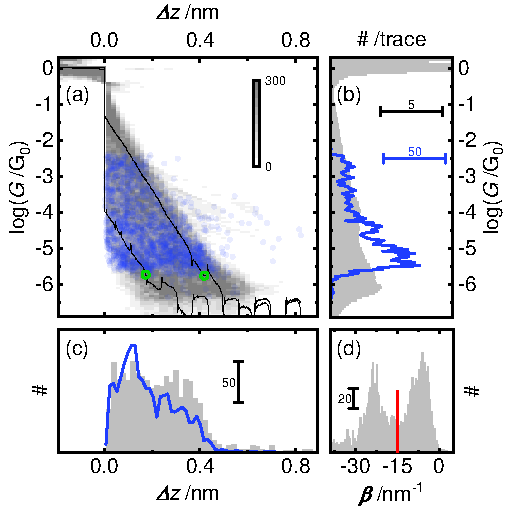
\includegraphics[width=\columnwidth,keepaspectratio,]{Fig_BPY_4K_tunnel}
\caption{Chow test applied to \bpycoldnumtun tunneling traces at \qty{4}{\K}. (a) \ac{2DH} of all molecular traces (gray). Scatter plot of Chow+ test choices of \ac{bp} (blue). (b) Conductance histograms of all tunneling traces (gray), and conductance values of Chow+ test results (blue). (c) \ac{plh} (gray), and histograms of displacement values of Chow+ test results  (blue). (d) Histogram of slopes of each trace \qty{1}{\angstrom} previous to \ac{bp} (gray). Red line marks threshold between mostly tunneling traces and mostly molecular traces used for classification in this study.}%
\label{fig:tunnel_cold}%
\end{figure}

Here it was important to note, there were a number of benefits of finding the \ac{bp}. One benefit was the increased resolution in the slope of the trace. Once the \ac{bp} of the trace was determined using the Chow+ test, the slope of each trace was determined by taking the slope of the previous \qty{1}{\angstrom} of the trace. This increased accuracy over conventional windowing methods by only using data that is in the molecular trace, without contamination from the steep portions following the Au-Au rupture or \ac{bp}. The increased accuracy allowed us to observe a sharp bimodal distribution in the slopes, Fig.~\ref{fig:tunnel_cold}(d), and sort the data into tunneling traces with steep slopes, and molecular traces with much flatter slopes.

Next the Chow+ test was applied to a data set of \ac{smbj} measurements on \ac{bpy} at \ac{rt}. Fig.~\ref{fig:BPY_rt}(a) was a \ac{2DH} of all traces in the data set, with \acp{bp} plotted in green. Two example traces were also plotted, with blue $\bigcirc$s to show the Chow+ test choice of \ac{bp}. The choices of \ac{bp} appeared to be accurate. The distribution of \acp{bp} was more clearly seen in histograms of conductance [Fig.~\ref{fig:BPY_rt}(b)] and displacements [Fig.~\ref{fig:BPY_rt}(c)]. It is well known \ac{bpy} at \ac{rt} exhibits a 2-step feature during junction elongation, and the conventional histograms in Figs.~\ref{fig:BPY_rt}(a) and (b) showed these features, while the Chow+ result was mostly insensitive to this behavior. This is a strength of using Chow+. Various molecules, e.g. \ac{bpy} here or the silane in the next section, are expected to exhibit a wide range of junction trajectories which may confound accurate estimates of $\overline{G}_{\text{mol}}$ and $\overline{z}_{\text{mol}}$. But eventually the molecular junction breaks, and this is likely to be the best estimate for $\overline{G}_{\text{mol}}$ and $\overline{z}_{\text{mol}}$. Fig.~\ref{fig:BPY_rt}(d) summarizes the estimates for $\overline{G}_{\text{mol}}$ and $\overline{z}_{\text{mol}}$, as determined by conventional \ac{1DGH}, \ac{plh}, and Chow+, for \ac{bpy} at \qty{4}{\K} [light gray and blue, from Fig.~\ref{fig:BPY_cold}(d)] and \ac{rt} (dark gray and green). The differences between Chow+ and conventional estimates for $\overline{G}_{\text{mol}}$ and $\overline{z}_{\text{mol}}$ in the \ac{rt} data was \qty{10.6}{\nano\siemens} and \qty{1}{\angstrom}. It is also noteworthy that the Chow+ test finds estimates which are shorter, and with lower conductance, than the conventional methods. This is not the case in the next example.
\begin{figure}[]%
	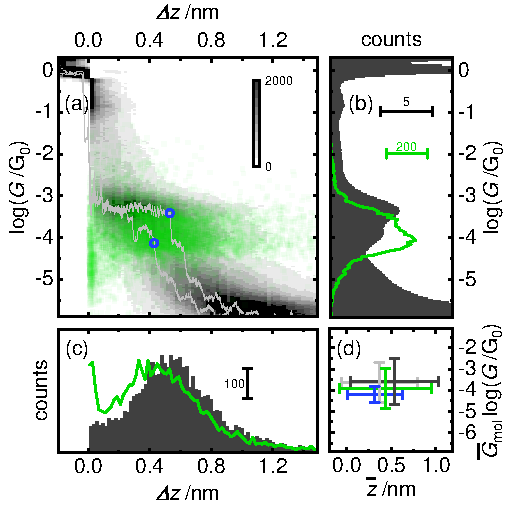
\includegraphics[width=\columnwidth,keepaspectratio,]{Fig_BPY_300K}
	\caption{Chow test applied to \bpyrtnum traces of \ac{bpy} at \ac{rt}. (a) \ac{2DH} of all molecular traces (gray). Scatter plots of Chow+ test choices of \ac{bp} (green). On top two example traces (light gray) with \ac{bp} (blue). (b) \ac{1DGH} of all traces (dark gray), and  histogram of conductance values of Chow+ test results (green). (c) \ac{plh} (gray), and histograms of displacement values of Chow+ test results (green). (d) Mean of Gaussian fit to \ac{1DGH} of all data between \qty{}{10^{-1.0}~\G} and \qty{}{10^{-4.4}~\G} (dark gray), and to conductances and displacements of Chow+ test results (green). Results for \qty{4}{\K} measurements (light gray and blue) included for comparison. Error bars are standard deviations.}%
	\label{fig:BPY_rt}%
\end{figure}


%---------------------------------------------------------%
\subsection{Complicated data: jumpy traces}
%---------------------------------------------------------%
The Chow+ identified a $\overline{G}_{\text{mol}}$ in \ac{bpy}, which has a downward sloping molecular plateau with steps, that was lower in conductance than the customary fit to the 1D conductance histogram peak.  This was the case for both cryogenic data with sharp features, and \ac{rt} data with thermally influenced features. We next applied Chow+ to a silane derivative at \ac{rt}.

\begin{figure}[]%
	\includegraphics[width=\columnwidth,keepaspectratio,]{Fig_Si4}
	\caption{Chow test applied to \num{\approx 19000} traces of a silane derivative at \ac{rt}. (a) 2D intensity plot of all molecular traces (gray). Scatter plots of Chow+ test choices of \ac{bp} (purple). On top an example trace (black) with \ac{bp} (purple $\bigcirc$). (b) Conductance histograms of all traces (purple), and conductance values of Chow+ test results (purple). (c) Plateau length histogram (gray), and histograms of displacement values of Chow+ test results (purple). (d) Mean of Gaussian fit to \ac{1DGH} of all data between \qty{}{10^{-0.5}~\G} and \qty{}{10^{-4.5}~\G}  and \ac{plh} (gray), and to conductances and displacements of Chow+ test results (purple). Error bars are standard deviations.}%
	\label{fig:Si}%
\end{figure}
The silane data set contained \sinum traces, from which \sinummol traces were identified as molecular traces, determined by the slope of the plateau \qty{0.5}{\angstrom} before the \ac{bp}. Fig.~\ref{fig:Si} plotted the results of the molecular traces. The data were previously reported in Ref.~\onlinecite{su2015stereoelectronic}. The frequent and large jumps in conductance were previously attributed to available Cauchy conformations during junction elongation. For the purposes of the present study, these jumps present a potential confounding feature in the data for our simplistic \ac{cpd}. Yet, results, plotted in Fig.~\ref{fig:Si}, were promising. Fig.~\ref{fig:Si}(a) showed \acp{bp} tightly distributed along the part of the \ac{2DH} where the majority of traces had straightened out any Cauchy folds before rupture. The example trace in Fig.~\ref{fig:Si}(a) was representative of this -- the \ac{bp} marked the end of the flat part of the trace. \Acp{bp} chosen at this point were likely to represent fully elongated junctions, comparable to geometries used by theory to model the junction. Conversely, values for $\overline{G}_{\text{mol}}$ derived from the \ac{1DGH}, Fig.~\ref{fig:Si}(b), will necessarily contain nature from the conductance jumps caused by the Cauchy conformations -- geometries other than straight elongated junctions. The narrowing of the conductance distribution between the conventional method (gray) and Chow+ (purple) was evident in Fig.~\ref{fig:Si}(b), though the distribution of displacements, Fig.~\ref{fig:Si}(c) appeared to change little. The summary in Fig.~\ref{fig:Si}(d) for $\overline{G}_{\text{mol}}$ and $\overline{z}_{\text{mol}}$ showed the standard deviation for the estimate of $\overline{G}_{\text{mol}}$ was halved between the conventional method and Chow+.


%---------------------------------------------------------%
\subsubsection{Sensitivity testing}
%---------------------------------------------------------%
It was important to understand how the \ac{bp} from the Chow test was dependent on the choice of parameters. The four parameters necessary to find the \ac{bp} presented here were
\begin{enumerate*}[(i)]
	\item search window ceiling,
	\item search window floor,
	\item number of backward points to search, and
	\item smoothing parameter.
\end{enumerate*}
The first two items were explored qualitatively in Fig.~\ref{fig:dummy_chow}. For the \ac{bpy} data at \qty{4}{\K}, in Fig.~\ref{fig:sensitivity}(a), the \ac{bp} search window ceiling was swept from \qty{}{10^{-0.4}~\G} to \qty{}{10^{-4.0}~\G} in steps of \num{0.2} on the $\log G/G_0$ scale. The distribution of \acp{bp} were then summarized using box plots, where the boxes span the \numrange{25}{75} percentiles, the vertical line marks the median, and the whiskers span the \num{1.5} standard deviation window; outliers are marked individually. Because no strong dependency was noticed, the value of \qty{}{10^{-2.4}~\G} (gray dashed line) was chosen as the ceiling threshold because it ignored superfluous data in the snap-back region. In Fig.~\ref{fig:sensitivity}(b) the \ac{bp} search window floor was swept from \qty{}{10^{-7.0}~\G} to \qty{}{10^{-3.6}~\G} in steps of \num{0.2} on the $\log G/G_0$ scale. In this case, there appeared to be a sensitivity to the choice of window floor. If the floor was chosen too low, in the noise region below \qty{}{10^{-6.3}~\G}, the \acp{bp} were frequently chosen within the noise region, where we do not expect a \ac{bp}. Conversely, if the floor was chosen too high, above \qty{}{\approx 10^{-5.0}~\G}, the \acp{bp} were predominantly chosen to be above the molecular plateau. The choice of \qty{}{10^{-5.7}~\G} (gray dashed line) was close to, but not within, the noise floor. In Fig.~\ref{fig:sensitivity}(c) the number of points to search backwards using the Chow+ algorithm was swept from \numrange{0}{10}. A value of \num{2} was chosen because it would contribute the smallest influence. Finally, the size of the smoothing window was swept from \numrange{5}{39} in Fig.~\ref{fig:sensitivity}(d). The \acp{bp} did not appear to be strongly dependent on this parameter. A choice of \num{21} was chosen to slightly increase calculation times, because the one-by-one search in the Chow test, as implemented here, was significantly more costly than the smoothing calculation. 
\begin{figure}[]%
	\includegraphics[width=\columnwidth,keepaspectratio,]{Fig_BPY_sensitivity}
	\caption{Sensitivity tests of the four parameters required to determine \acp{bp} using Chow+ summarized in box plots applied to \ac{bpy} data at \qty{4}{\K}. Results of the search window (a) ceiling, (b) floor, (c) backward search size, and (d) smoothing parameter. Boxes are \numrange{25}{75} percentiles, whiskers are \num{1.5} standard deviations, and vertical line is the distribution median; outliers plotted individually. Black arrows show final choice for parameter value.}%
	\label{fig:sensitivity}%
\end{figure}

Similar sensitivity tests were performed for \ac{bpy} at \ac{rt} (Fig.~\ref{fig:sensitivityRT}) and silane (Fig.~\ref{fig:sensitivitySi}). Results were similar to \ac{bpy} at \qty{4}{\K}.
\begin{figure}[]%
	\includegraphics[width=\columnwidth,keepaspectratio,]{Fig_BPY_300K_sensitivity}
	\caption{Sensitivity tests of the four parameters required to determine \acp{bp} using Chow+ summarized in box plots applied to \ac{bpy} data at \ac{rt}. Results of the search window (a) ceiling, (b) floor, (c) backward search size, and (d) smoothing parameter. Boxes are \numrange{25}{75} percentiles, whiskers are \num{1.5} standard deviations, and vertical line is the distribution median; outliers plotted individually. Black arrows show final choice for parameter value.}%
	\label{fig:sensitivityRT}%
\end{figure}

\begin{figure}[]%
	\includegraphics[width=\columnwidth,keepaspectratio,]{Fig_Si4_sensitivity}
	\caption{Sensitivity tests of the four parameters required to determine \acp{bp} using Chow+ summarized in box plots applied to silane data. Results of the search window (a) ceiling, (b) floor, (c) backward search size, and (d) smoothing parameter. Boxes are \numrange{25}{75} percentiles, whiskers are \num{1.5} standard deviations, and vertical line is the distribution median; outliers plotted individually. Black arrows show final choice for parameter value.}%
	\label{fig:sensitivitySi}%
\end{figure}


\section{Conclusion}

We have presented a proof-of-concept for applying \ac{cpd} to determine the molecular conductance and displacement of a \ac{smbj} trace. In every example we have analyzed, the resulting summary statistics provide estimates for $\overline{G}_{\text{mol}}$ with smaller standard deviation, typically by half, compared to the conventional \ac{1DGH} method.

In this study we utilized the Chow test because of its simplicity. The Chow test has a couple of shortcomings; its conventional implementation is slow, and it assumes as the null hypothesis that a single unit root exists, even if there are more than one, or none at all. In most \ac{smbj} traces this is a safe assumption, and we have presented results on molecules which exhibit more than one apparent break points without excessive complications. In the case of multiple break points, other \ac{cpd} algorithms may be better suited. Most notably, Bayesian methods including the Hidden Markov Model approach, was not presented here. One reason for this choice was to present a counterpoint to \ac{ml}, based on the premise that, when faced with an intractable problem, most researchers do not need more complicated \ac{ml}, only better statistics. Contrary to most, or all, \ac{ml} methods, Chow+ requires four physically meaningful tuning parameters, three of which (window ceiling and floor, and smoothing window) are typically applied during \ac{ml} workflow as well. The fourth is \textit{ad hoc}, but does not need to be used at all, and when it is used, provides only small corrections to the algorithm.

The strengths of applying \ac{cpd} to determine $\overline{G}_{\text{mol}}$ and $\overline{z}_{\text{mol}}$ are manyfold. Determining a single scalar value from each trace will help with \ac{ml} approaches, which are currently searching around for effective dimensionality reduction devices. A single scalar value rom each trace can be plotted in a timeseries, providing researchers with a tool to monitor experiments online, and poll real-time statistics. With improvements, methods to search for multiple break points will be useful for studying in further detail molecules like \ac{bpy} and silane. 


%\section{extra results}
%%
%
%%---------------------------------------------------------%
%\subsection{Expanding mean of the \acp{bp}\label{sec:exp_mean}}
%%---------------------------------------------------------%
%%\todo[inline]{this section becomes difficult to support with current results}
%Using the \acp{bp} of the experiment provided a new way to describe the progress of the experiment. Because the \ac{1DGH} poorly described $\overline{G}_{\text{mol}}$ in cases when the plateau was highly sloped, and a fit to a Gaussian was only possible after a large amount of data was acquired, we wished to see how quickly the mean conductance of the \acp{bp} converged to an experimental $\overline{G}_{\text{mol}}$. Returning to the \qty{4}{\K} results, Fig.~\ref{fig:timeseries4K}(a) plotted the expanding mean as each new trace was added to the data set. To visualize how much this deviated from the final sample mean, this was subtracted and the absolute deviation was plotted. Furthermore, the expanding standard error (standard deviation of first $n$ elements divided by $\sqrt(n)$) was plotted as a red shaded region to give a scale of the deviation. Generally, if the deviation stays within the standard error window, each new trace is similar to all the previous traces, and provides little new information; contrarily, if the deviations vary wildly, then a stable sample mean has not been reached. From the previous section, we knew a large number of tunneling traces contributed to the data set, so results were plotted for all traces [Fig.~\ref{fig:timeseries4K}(a)], and only molecular traces [Fig.~\ref{fig:timeseries4K}(b)]. 
%%Above Fig.~\ref{fig:timeseries4K}(a) a rug is plotted to indicate which indices were labeled molecular traces, based on the plateau slope as in the previous section. 
%\begin{figure}[]%
%	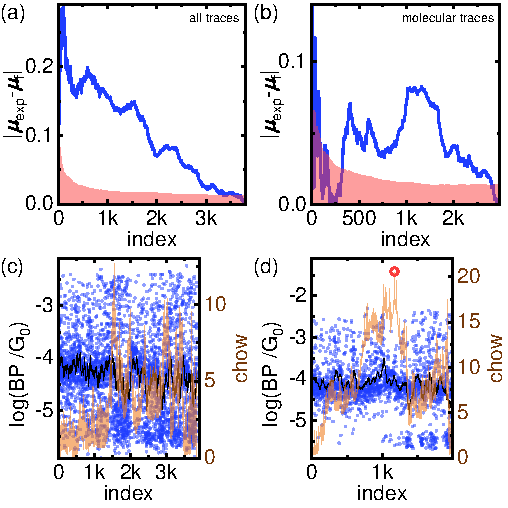
\includegraphics[width=\columnwidth,keepaspectratio,]{Fig_BPY_timeseries_4K}
%	\caption{Expanding mean minus final sample mean of \ac{bpy} \acp{bp} at \qty{4}{\K} for (a) the entire data set and (b) only molecular traces (blue), and expanding standard error (red). \acp{Bp} in order of acquisition (blue) and after a rolling mean with window size of \num{40} is applied as an aid for the eye (black), and Chow score for structural break in timeseries (orange), for (c) all traces and (d) molecular traces.}%
%	\label{fig:timeseries4K}%
%\end{figure}
%
%Conventionally, \acp{1DGH} from tunneling traces have a weak influence on the results of a total \ac{1DGH} from an entire experiment, because there are few counts in the molecular window. Historically, this influence has been largely ignored. On the other hand, tunneling trace \acp{bp} contribute equally to the distribution of the entire experiment. For this reason, it might not be surprising that Fig.~\ref{fig:timeseries4K}(a) does not converge to an asymptotic deviation around the mean. However, even after removing tunneling traces from the distribution, Fig.~\ref{fig:timeseries4K}(b), the expanding mean does not asymptote to a small deviation quickly, and the the scatter of \acp{bp} do not appear to be regular.
%
%Results were different for \ac{bpy} at \ac{rt}. In this case, plotted in Fig.~\ref{fig:timeseries300K}(a), the expanding deviation was much smaller, and the expanding mean eventually appeared to asymptote inside the deviation window. Furthermore, the timeseries of the \acp{bp}, Fig.~\ref{fig:timeseries300K}(b) appeared to have a regular variance around a single mean.
%
%%Results were different for \ac{bpy} at \ac{rt}. In this case, the expanding mean, Fig.~\ref{fig:timeseries300K}(a), approached an asymptote inside the expanding standard error quickly, within approximately \num{100} traces, as evident in the inset Fig.~\ref{fig:timeseries300K}(a). The time series of the \acp{bp}, Fig.~\ref{fig:timeseries300K}(b) appeared to have a regular variance around a single mean.
%\begin{figure}[]%
%	\includegraphics[width=\columnwidth,keepaspectratio,]{Fig_BPY_timeseries_300K}
%	\caption{(a) Expanding mean minus final sample mean of \ac{bpy} \acp{bp} at \ac{rt}, and expanding standard error (red). (b) \acp{Bp} in order of acquisition (blue) and after a rolling mean with window size of \num{40} is applied as an aid for the eye (black), and Chow score for structural break in timeseries (orange).}%
%	\label{fig:timeseries300K}%
%\end{figure}
%
%
%%---------------------------------------------------------%
%\subsection{Stationarity of the \acp{bp} over the experiment\label{sec:stationarity}}
%%---------------------------------------------------------%
%The previous section showed the timeseries of \qty{4}{\K} and \ac{rt} \acp{bp} appeared qualitatively different. The \qty{4}{\K} \acp{bp} vary more, and appear not to vary around a single mean. On the other hand, the \ac{rt} \acp{bp} appeared to have a regular variance around a single mean. In this section we wish to quantify the question "does the timeseries vary around a single mean with a constant standard deviation?" This is a question of stationarity. If the timeseries is not stationary, then we can apply the Chow test to investigate the structural break. Earlier we introduced the Chow test as a way to find a structural break in a timeseries, and applied it to individual traces to determine the structural break with the assumption that the structural break existed in the data. For the timeseries of \acp{bp} as an experiment progresses there is no such assumption - there may be no structural break, or there may be many. Therefore, first we must establish that a structural break exists, before employing the Chow test to estimate where the break is. 
%
%A number of tests have been developed to test for a unit root or structural break,\cite{Elliott1992, PHILLIPS1988} mostly built upon the \ac{df} test.\cite{Dickey1979}\todo{we could include the mathssss for this here} But, like the Chow test, they assume the unit root or structural break exists, and are biased towards that conclusion. The \ac{kpss} test has stationarity as the null hypothesis, and unit root as the alternative hypothesis.\cite{Kwiatkowski1992} In the \ac{kpss} test the data is modeled as a sum,
%\begin{equation}\label{eq:kpss}
%	y_t = \xi t + r_t + \varepsilon_t,
%\end{equation}
%of a deterministic trend, $\xi$, a random walk, $r_t$, and a stationary error, $\varepsilon_t$, and then uses the Lagrangian multiplier test to \todo[inline]{finish this}. By applying the \ac{kpss} test to our timeseries, we get a score for how likely the timeseries is stationary. If it fails the test, then we can conclude that there is a unit root in the data, and then search for it with the Chow test. Critically, the literature agrees \ac{kpss} should be used in conjunction with a test for unit root. Here we utilize the \ac{dfgls} test for this, which is an advanced version of the \ac{df} test. 
%
%The \ac{kpss} test was applied to both timeseries [Fig.~\ref{fig:timeseries4K}(d) and Fig.~\ref{fig:timeseries300K}(b)]. We assumed the timeseries had no regular trend, $\xi=0$ in Eq.~\ref{eq:kpss}. The results are summarized in Table~\ref{tab:kpss}.
%\begin{table}
%	\caption{\label{tab:kpss} }
%	\begin{ruledtabular}
%		\begin{tabular}{rlrrl}
%			Experiment & Test                                                                                             & Statistic   & p-value   & Null\footnote{\qty{95}{\percent} confidence} \\
%			BPY @ \qty{4}{\K}   & \ac{kpss}\footnote{\ac{kpss}: null hypothesis is timeseries is stationary}               & \num{1.220}     & \num{0.001}     & Reject               \\
%			BPY @ \qty{4}{\K}   & \ac{dfgls}\footnote{\ac{dfgls}: null hypothesis is timeseries has a unit root}          & \num{-5.070}     & \num{0.000}     & Reject        \\
%			BPY1\footnote{up to trace \num{1293} } @ \qty{4}{\K}   & \ac{kpss}                                              & \num{0.172}      & \num{0.328}    & Accept        \\
%			BPY1 @ \qty{4}{\K}   & \ac{dfgls}                                                                             & \num{-2.982}   & \num{0.003}      & Reject        \\
%			%BPY1 @ \qty{4}{\K}   & \ac{kpss} trend\footnote{\ac{kpss} with linear trend}                                 & \num{0.167}      & \num{0.032}      & Reject         \\
%			%BPY1 @ \qty{4}{\K}   & \ac{dfgls} trend\footnote{\ac{dfgls} with linear trend}                               & \num{-32.429}      & \num{0.000}     & Reject      \\
%			BPY2\footnote{trace \num{1168} and after} @ \qty{4}{\K}   & \ac{kpss}                                            & \num{0.771}    & \num{0.009}       & Reject        \\
%			BPY2 @ \qty{4}{\K}   & \ac{dfgls}                                                                               & \num{-4.088}     & \num{0.000}      & Reject        \\
%			BPY @ \ac{rt}   & \ac{kpss}                                                                                     & \num{1.133}    & \num{0.001}       & Reject        \\
%			BPY @ \ac{rt}   & \ac{dfgls}                                                                                     & \num{-4.122}    & \num{0.000}       & Reject        \\
%		\end{tabular}
%	\end{ruledtabular}
%\end{table}
%%From Table~\ref{tab:kpss}, the interpretation of the \ac{bpy} \ac{bp} timeseries measured at \ac{rt} was that the hypothesis that the timeseries has a unit root was rejected, and the hypothesis that the timeseries was stationary was accepted. These are consistent between each other, and with the qualitative assessment that the timeseries appeared to have a single mean and standard deviation throughout. 
%
%From Table~\ref{tab:kpss}, the interpretation of the \ac{bpy} \ac{bp} timeseries measured at \ac{rt} was that the hypothesis that the timeseries has a unit root was rejected, and the hypothesis that the timeseries was stationary was accepted. These are consistent between each other, and with the qualitative assessment that the timeseries appeared to have a single mean and standard deviation throughout. 
%
%The interpretation of the \ac{bpy} \ac{bp} timeseries measured at \qty{4}{\K} was more nuanced. Both hypotheses were rejected for the entire timeseries of molecular traces. This suggested there may be at least one unit root, but we are not completely confident in this interpretation. To investigate further, the Chow test was applied to the timeseries, Fig.~\ref{fig:timeseries4K}(d), which identified a \ac{bp} at trace \num{1293}. The timeseries was split in two at this trace, and retested with \ac{kpss} and \ac{dfgls}. The results were summarized in Table~\ref{tab:kpss}. The test for stationarity on the second segment was accepted, but rejected on the first segment. The test for unit root was rejected for both segments. 
%
%Tests for stationarity on the two segments were accepted, and tests for unit root were rejected. This suggested that the experiment performed at \qty{4}{\K} may have been sampling from one mean conductance for some time, and then sometime around trace \num{1293}, transitioned to a different mean conductance, while the \ac{rt} experiment either sampled from a single mean conductance the entire experiment, which is unlikely, or sampled from such a large number of mean conductances throughout that the central limit theorem was in play.
%
%The result that the \ac{rt} data sampled from a large number of distributions, while the \qty{4}{\K} data only sampled from a small number of distributions is key result which is only apparent when looking at the data sets as timeseries evolving in time. Conventional summary histograms cannot capture this.



%The \ac{odt} data set of \qty{\approx 16000} traces was determined to have \qty{\approx 6000} molecular traces, determined by the plateau length. Fig.~\ref{fig:ODT_rt} plotted the results.
%\begin{figure}[]%
%\includegraphics[width=\columnwidth,keepaspectratio,]{Fig_ODT_rt}
%\caption{Chow test applied to \qty{\approx 6000} traces of \ac{odt} at \ac{rt}. (a) 2D intensity plot of all molecular traces (gray). Scatter plots of Chow+ test choices of \ac{bp} (blue). On top an example trace (black) with \ac{bp} (blue $\bigcirc$). (b) Conductance histograms of all traces (dark gray), and conductance values of Chow+ test results (blue). (c) Plateau length histogram (gray), and histograms of displacement values of Chow+ test results (blue). }%
%\label{fig:ODT_rt}%
%\end{figure}

%One striking improvement the Chow+ method made over the conventional methods was to reduce the standard deviation in the conductance by half.

%The result that at \qty{4}{\K} the expanding mean of the conductance appeared to not asymptote, at least for the data available, while at \ac{rt} the same metric reached asymptote within \qty{\approx 500} traces suggested a couple of possible interpretations:
%\begin{enumerate*}[(i)]
%\item at \qty{4}{\K} it takes longer for the experiment to stabilize, while at \ac{rt} the experiment stabilizes quickly, or
%\item at \qty{4}{\K} the experiment is sampling from a small number of different distributions, while at \ac{rt} the number of distributions is so large, it is effectively continuous.\label{item:exp}
%\end{enumerate*}
%These two separate interpretations suggest their own implications. The current study is not concerned with best practices for experimental designs, but we will return to this momentarily in the conclusion. Instead, we will focus on interpretation \ref{item:exp}. In this scenario, we can ask the question: does the \qty{4}{\K} data sample from one distribution for a while, and then switch to sampling from another? This is suggested by the results in \S\ref{sec:exp_mean} because the means of the separate subgroups in Fig.~\ref{fig:timeseries4K}(d) vary significantly among each other and from the final sample mean.
%
%The question we are asking of the data is this: is the data stationary, or does the data contain a structural break or unit root? We have already introduced the Chow test is a basic test for determining where the structural break is, and to what confidence. Furthermore, there is a suite of tests for asking "is there a structural break" or "is there a unit root" in the series. But asking "is the data stationary" calls for a separate metric because any statistic that asks "is there a structural break" will be biased towards that null hypothesis. 

%\begin{figure}[]%
%\includegraphics[width=\columnwidth,keepaspectratio,]{Fig_Exp_Mean_4K}
%\caption{Evolution of the \ac{bp} sample mean as new data is added to the set. (a) Expanding mean minus final sample mean of \qty{4}{\K} \ac{bpy} with rug indicating which indices were identified as molecular traces. Red shaded region indicates region within the standard error. (b) Expanding mean minus final sample mean of seven consecutive subgroups of the data, each containing \qty{512} traces. (c) Expanding mean minus final sub-sample mean of only molecular traces. (d) Expanding mean minus final sub-sample mean of three consecutive sub-groups of only molecular traces.}%
%\label{fig:means4K}%
%\end{figure}




%To visualize this, we arbitrarily broke the data in Fig.~\ref{fig:means4K}(a) into consecutive groups of \qty{512} traces and re-calculated the expanding mean for each group. Each group was offset by the entire data set's sample mean. The results were plotted in Fig.~\ref{fig:means4K}(b). Each sub-group had a distinct deviation from the final mean, meaning if only that sub-group were used, there would be disagreement of as much as \qty{\approx 0.5} on the $log(G/G_0)$ scale. 



%This result becomes interesting when compared to results at \ac{rt}. Fig.~\ref{fig:means300K}(a) plots the expanding mean of the \ac{bpy} results measured at \ac{rt}. Firstly, it is significant that the expanding mean reaches and maintains inside the window of the standard error. In other words, each new data point added to the data set changes the new sample mean by less than the the standard error. The key takeaway from this is that, if the experiment were stopped at \qty{\approx 500} traces, the conclusion from the experiment would not change.\todo[inline]{reword this}

%\begin{figure}[]%
%\includegraphics[width=\columnwidth,keepaspectratio,]{Fig_Exp_Mean_300K}
%\caption{Evolution of the \ac{bp} sample mean as new data is added to the set. (a) Expanding mean minus final sample mean of \qty{300}{\K} \ac{bpy}. Red shaded region indicates region within the standard error. (b) Expanding mean minus final sample mean of seven consecutive subgroups of the data, each containing \qty{512} traces. (c) \acp{Bp} (blue) in order of acquisition; \acp{Bp} after applying a rolling mean with window size of \qty{100} (gray); Chow test applied to each trace in the sequence (orange). (d) Expanding mean minus final sub-sample mean of three consecutive sub-groups of only molecular traces.}%
%\label{fig:means300K}%
%\end{figure}
%
%This conclusion is reinforced when the expanding mean of sub-groups of \qty{512} traces are calculated. Any single sub-group yields a similar mean, within \qty{\approx 0.1} on the $log(G/G_0)$ scale.\todo[inline]{probably need to quantify these statements}
%



%Because the Chow test performs a series of linear regressions, there was a concern that it may perform differently when the \ac{bp} was located near the edges of the data, and the test may be sensitive to how much noise data was retained in the trace. To validate these conditions, we tested the Chow test on a series of idealized data sets with clear structural breaks. Fig.~\ref{fig:chow} shows the Chow test applied to data which contains one [(a) and (b)], two [(c) and (d)], and three [(e) and (f)] \acs{bp}. Data of this form is common in econometrics, where the Chow test was first developed. As predicted, the test preferred the center of the data window. This preference was only consequential in the dummy data with three \acs{bp} [Figs.~\ref{fig:chow}(e) and (f)]. In this case, moving the breaking features within the data window can switch the location of the \ac{bp}, as determined by the Chow test, from the third break in the sequence, to the first. In all other cases, the \ac{bp} was less sensitive to the location within the data window.
%\begin{figure}[ht]%
%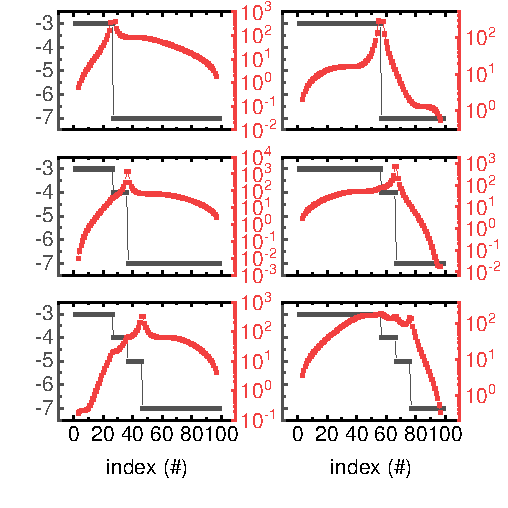
\includegraphics[width=\columnwidth,keepaspectratio,]{Fig_Chow}
%\caption{Chow test applied to dummy data.}%
%\label{fig:chow}%
%\end{figure}

%A subtle question in \ac{smbj} measurements is when to conclude an experiment, and how much bias does this choice impart on the conclusions.

%In the case of Figs.~\ref{fig:timeseries4K}(a) and (b), the inclusion of tunneling traces has the potential to confound the conclusions, because, unlike the case when 1D conductance histograms are used, when the \acp{bp} are used, the tunneling traces contribute equally to the final distribution. Therefore, in Figs.~\ref{fig:timeseries4K}(c) and (d), the tunneling traces were removed from the expanding mean, and the sub-group sample mean was used to offset the result. However, the conclusion was not improved --- the expanding mean in Fig.~\ref{fig:timeseries4K}(c) never reached an asymptote, and the subgroups in Fig.~\ref{fig:timeseries4K}(d) had a similarly wide spread of final deviations from the sample mean of all molecular traces.

%We next applied the Chow test to two test molecules already studied in the literature. Following the lessons learned above, we windowed each trace to focus the Chow test on the molecular region. Based on the total 1D conductance histogram, we determined that the molecular plateau in most traces began after \qty{}{10^{-2}~\G} and ended following \qty{}{10^{-4.5}~\G}. This imparts some degree of subjectivity, and requires some for-knowledge of the data being studied, but...\todo[inline]{finish this} \todo[inline]{it might be necessary to do sensitivity testing in SM}
%
%
%Changes in conductance of this magnitude was reported in single-molecule switches.\cite{Higgins2017, Huang2017}. 
%
%
%Two simplifications were necessary to create Fig.~\ref{fig:means}(a). First, only the molecular traces, the traces which contributed to Figs.~\ref{fig:BPY_cold}~and~\ref{fig:BPY_rt} were included. Tunneling traces complicated the utility of figure. However, it was possible to envision an automated algorithm, running alongside data acquisition, to sort between molecular traces and tunneling traces in real-time. The second simplification was to randomize the traces. It has been shown that the quality of experiments changed throughout an experiment.\cite{Magyarkuti2017} This nuance also complicated the utility of the figure, and this behavior of the experiment was much more difficult for the experimentalist to control. With these simplifications in mind, evolving means in Fig.~\ref{fig:means}(a) appear to converge in under \qty{1000} traces to a steady mean. 
%
%Furthermore, it seemed clear the two experiments were not converging to a single value. Fig.~\ref{fig:means4K}(b) plotted the scaled \acp{bp} conductance histograms together. On the same conductance scale, and when the histograms were scaled to unity, the \qty{4}{\K} histogram fell within the lower half of the \ac{rt} histogram. This suggested the \ac{rt} molecular junctions had access to all the degrees of freedom the \qty{4}{\K} junctions had, and also many more. The distribution of \ac{rt} \acp{bp} even began to show the bimodal distribution customary in \ac{bpy} conductance histograms.
%
% The same analysis was plotted with tunneling traces removed.\todo[inline]{add SI, I guess, or just add another figure}. The data contributing to Fig.~\ref{fig:timeseries4K}(a) were clearly being drawn from at least two separate distributions. 

\begin{acknowledgments}
	This project has received funding from the European Union’s Horizon 2020 research and innovation programme under the Marie Skłodowska-Curie grant agreement No 884741.
\end{acknowledgments}

\bibliographystyle{apsrev4-2}
\bibliography{library}

\end{document}
